\documentclass[xetex,table]{beamer}

\usepackage{fontspec}
\usepackage[autostyle]{csquotes}
\usepackage{hyperref}
\usepackage{color}
\usepackage{setspace}
\usepackage{listings}
\usepackage{minted}

\usetheme{metropolis}

\title{Elaborazione dati dalla riga di comando}
\author{Luca Ceresoli}
\date{}

\begin{document}

\maketitle

\section{Elaborare dati}

\begin{frame}
  \frametitle{Sistemi per elaborare dati}
  Informatica = elaborazione automatica delle informazioni
  \begin{itemize}
  \item Database relazionali
  \item Spreadsheet
  \item Software ad-hoc
  \item \dots
  \item La riga di comando
  \end{itemize}
\end{frame}

\section{La riga di comando}

\begin{frame}
  \frametitle{La riga di comando}
  \begin{itemize}
  \item Strumento classico, nato ai tempi dai "terminali"
  \item Prompt: richiede un "comando", lo esegue, torna al prompt
  \item Esistono migliaia di possibili comandi
  \item Molto spartana, molto potente
    \begin{itemize}
    \item Presente su praticamente ogni sistema UNIX-like
    \item Utilizzabile su sistemi poco carrozzati...
    \item ...o remoti, con connessioni lentissime
    \end{itemize}
  \end{itemize}
\end{frame}

\begin{frame}
  \frametitle{Standard input, standard output, standard error}
  \begin{center}
    \includegraphics[height=0.6\textheight]{images/process.pdf}
  \end{center}
\end{frame}

\begin{frame}
  \frametitle{Visualizzare i dati}
  \begin{itemize}
  \item \texttt{cat}
  \item \texttt{less}
  \item \texttt{wc}
  \item \texttt{head}, \texttt{tail}
  \item Demo!
  \end{itemize}
\end{frame}

\begin{frame}
  \frametitle{Semplici elaborazioni}
  \begin{itemize}
  \item \texttt{sort}
  \item \texttt{cut}
  \item Demo!
  \end{itemize}
\end{frame}

\section{grep}

\begin{frame}
  \frametitle{grep}
  \begin{itemize}
  \item Filtra le righe, lasciando passare solo le linee che
    corrispondono a un criterio (pattern)
  \item Utilizzo base:
    \begin{itemize}
    \item \texttt{grep {\em PATTERN} file1 file2 file3}
    \item \texttt{grep {\em PATTERN}}
      \begin{itemize}
        \item Filtra lo standard input
      \end{itemize}
    \end{itemize}
  \item Demo!
  \end{itemize}
\end{frame}

\begin{frame}
  \frametitle{grep: varianti}
  \begin{itemize}
  \item Tipi di pattern:
    \begin{itemize}
    \item \texttt{grep {\bf -F} \emph{PATTERN}} --- Ricerca esatta
    \item \texttt{grep {\bf -G} \emph{PATTERN}} --- Basic regular expressions
    \item \texttt{grep {\bf -E} \emph{PATTERN}} --- Extended regular expressions
    \end{itemize}
  \end{itemize}
\end{frame}

\begin{frame}
  \frametitle{grep: opzioni aggiuntive}
  \begin{itemize}
  \item \texttt{-i}: case insentitive
  \item \texttt{-w}: solo parole intere
  \item \texttt{-v}: invert selection: mostra righe {\em non} corrispondenti
  \item \texttt{-l}: mostra solo i nomi dei files corrispondenti
  \item Demo!
  \end{itemize}
\end{frame}

\section{La pipeline}

\begin{frame}
  \frametitle{La pipeline}
  \begin{itemize}
  \item Simbolo: |
  \item Permette di collegare comandi "in catena"
  \item Principio UNIX: ogni software svolge una funzione
    \begin{itemize}
    \item La svolge in modo flessibile ed efficiente
    \item Si integra con altri strumenti che svolgono altre funzioni
    \end{itemize}
  \end{itemize}
\end{frame}

\begin{frame}
  \frametitle{La pipeline}
  Esempio: \texttt{ls -l | grep txt}
  \begin{center}
    \includegraphics[height=0.6\textheight]{images/pipeline.pdf}
  \end{center}
\end{frame}

\begin{frame}
  \frametitle{Semplici elaborazioni con la pipeline}
  \begin{itemize}
  \item \texttt{uniq}
  \item \texttt{tr}
  \item Demo!
  \end{itemize}
\end{frame}

\section{Espressioni regolari}

\begin{frame}
  \frametitle{Espressioni regolari}
  Espressioni regolari = Regular expressions = regexp
  \begin{itemize}
  \item Un linguaggio per descrivere un pattern
  \item Elabora una stringa (= sequenza di caratteri)
    \begin{itemize}
    \item Esito: match o non match
    \end{itemize}
  \item Usato da grep, sed e vari altri strumenti
  \end{itemize}
\end{frame}

\begin{frame}
  \frametitle{Sottostringa}
  \begin{itemize}
  \item Sottostringa: regexp senza caratteri speciali
    \begin{itemize}
    \item Esempio: ``in''
    \item Significato: tutte le stringhe contenenti ``in''
    \item Match: ``{\bf in}'', ``L{\bf in}ux'', ``P{\bf in}guino''
    \item No match: ``MacOS'', ``UNIX''
    \end{itemize}
  \end{itemize}
\end{frame}

\begin{frame}
  \frametitle{Qualsiasi carattere}
  \begin{itemize}
  \item Punto: qualsiasi carattere
    \begin{itemize}
    \item Esempio: ``.in.x''
    \item Significato: tutte le stringhe contenenti un carattere
      qualsiasi, poi ``in'', poi un carattere qualsiasi, poi ``x''
    \item Match: ``{\bf Linux}'', ``{\bf Minix}'', ``GNU {\bf Linux}''
    \item No match: ``inox'', ``Linoox''
    \end{itemize}
  \end{itemize}
\end{frame}

\begin{frame}
  \frametitle{Un carattere da un elenco}
  \begin{itemize}
  \item \texttt{[{\em caratteri}]}: un carattere da un elenco
    \begin{itemize}
    \item Esempio: ``\texttt{c[ao]sa}''
    \item Match: ``{\bf casa}'', ``{\bf cosa}''
    \item No match: ``cisa''
    \end{itemize}
  \item \texttt{[{\em x-y}]}: un range di caratteri
    \begin{itemize}
    \item Esempio: ``\texttt{casa[a-z]}''
    \item Match: ``rin{\bf casar}e'', ``{\bf casal}e''
    \item No match: ``casa''
    \end{itemize}
  \item \texttt{[\^{}{\em caratteri}]}: un carattere non nell'elenco
    \begin{itemize}
    \item Esempio: ``\texttt{casa[\^{}a-z]}''
    \item Match: ``{\bf casa!}'', ``{\bf casa }dolce casa''
    \item No match: ``casa'', ``casale''
    \end{itemize}
  \end{itemize}
\end{frame}

\begin{frame}
  \frametitle{Inizio e fine stringa}
  \begin{itemize}
  \item '\^{}': inizio stringa
  \item '\${}': fine stringa
    \begin{itemize}
    \item Esempio: ``\^{}casa\${}''
    \item Match: ``{\bf casa}''
    \item No match: ``casale'', ``rincasa''
    \end{itemize}
  \end{itemize}
\end{frame}

\begin{frame}
  \frametitle{Stringa opzionale}
  \begin{itemize}
  \item '?': zero o una volta
    \begin{itemize}
    \item Esempio: ``https?://''
    \item Match: ``{\bf http://}'', ``{\bf https://}''
    \item No match: ``httpss://''
    \end{itemize}
  \end{itemize}
\end{frame}

\begin{frame}
  \frametitle{Ripetizioni}
  \begin{itemize}
  \item '*': zero o più volte
    \begin{itemize}
    \item Esempio: ``0*123''
    \item Match: ``{\bf 123}'', ``{\bf 0123}'', ``{\bf 000123}'', ``0.{\bf 123}45''
    \item No match: ``023'', ``000012''
    \end{itemize}
  \item '+': una o più volte
    \begin{itemize}
    \item Esempio: ``0+123''
    \item Match: ``{\bf 0123}'', ``{\bf 000123}''
    \item No match: ``123'', ``023'', ``000012'', ``0.12345''
    \end{itemize}
  \end{itemize}
\end{frame}

\begin{frame}
  \frametitle{Sottoespressione}
  \begin{itemize}
  \item '( )': sequenza di caratteri da considerarsi come un elemento
    unico
    \begin{itemize}
    \item Esempio: ``http://(www.)?example.com''
    \item Match: ``{\bf http://www.example.com}'', ``{\bf http://example.com}''
    \item No match: ``http://ww.example.com''
    \end{itemize}
    \item Usato anche per la {\em substitution}
  \end{itemize}
\end{frame}

\begin{frame}
  \frametitle{Alternativa}
  \begin{itemize}
  \item '|': una sequenze tra varie possibili
    unico
    \begin{itemize}
    \item Esempio: ``www.example.(com|org|net)''
    \item Match: ``http://{\bf www.example.com}'', ``{\bf www.example.org}''
    \item No match: ``www.example.it''
    \end{itemize}
  \end{itemize}
\end{frame}

\begin{frame}
  \frametitle{Espressioni regolari: conclusioni}
  \begin{itemize}
  \item Sono uno strumento potente, ma insidioso
  \item Da verificare sempre con cura
    \begin{itemize}
    \item \texttt{grep -E '{\em regexp}'}
    \item strumenti online (es: \url{http://regexr.com/})
    \item Attenzione a falsi positivi e falsi negativi
    \end{itemize}
  \end{itemize}
\end{frame}

\section{sed}

\begin{frame}
  \frametitle{sed = the Stream EDitor}
  \begin{columns}
    \column{0.6\textwidth}
    Per ogni linea di input:
    \begin{itemize}
    \item Memorizza la riga nel {\em pattern space}
    \item Esegue il {\em sed script} che modifica il pattern space
    \item emette il {\em pattern space}
    \end{itemize}
    \column{0.4\textwidth}
    \begin{center}
      \includegraphics[height=0.6\textheight]{images/sed1.pdf}
    \end{center}
  \end{columns}
\end{frame}

\begin{frame}
  \frametitle{sed script}
  Sed script = una o più terne:
  \begin{itemize}
  \item address (opzionale): se corrisponde, il comando viene eseguito
  \item comando: una lettera
  \item eventuali parametri del comando
  \end{itemize}
  \begin{center}
    \includegraphics[height=0.6\textheight]{images/sed2.pdf}
  \end{center}
\end{frame}

\begin{frame}
  \frametitle{sed script}
  \begin{itemize}
  \item Address
    \begin{itemize}
    \item Numero di riga
    \item Range di numeri di riga
    \item \texttt{/{\em regexp}/}
    \end{itemize}
  \item Comandi principali
    \begin{itemize}
    \item \texttt{s/\emph{regexp}/\emph{replacement}/} --- sostituzione
    \item \texttt{d} --- elimina la riga
    \end{itemize}
  \item Demo!
  \end{itemize}
\end{frame}

\section{awk}

\begin{frame}
  \frametitle{awk}
  \begin{itemize}
  \item Linguaggio di programmazione progettato per estrarre ed
    elaborare dati
  \item Struttura simile a \texttt{sed}: coppie pattern + comando
  \item Ma il comando è un vero programma
    \begin{itemize}
    \item linguaggio simile al C
    \end{itemize}
  \end{itemize}
\end{frame}

\begin{frame}
  \frametitle{Flusso di esecuzione}
  \begin{columns}
    \column{0.4\textwidth}
    Per ogni linea di input:
    \begin{itemize}
    \item Memorizza la riga ({\em record})
      \begin{itemize}
      \item E i singoli campi
      \end{itemize}
    \item Esegue l'{\em awk script}
    \end{itemize}
    \column{0.6\textwidth}
    \begin{center}
      \includegraphics[height=0.4\textheight]{images/awk-flow.pdf}
    \end{center}
  \end{columns}
\end{frame}

\begin{frame}[fragile]
  \frametitle{awk script}
  Sed script = una o più coppie:
  \begin{minted}{awk}
condizione { azione }
  \end{minted}
    \begin{center}
      \includegraphics[height=0.4\textheight]{images/awk-script.pdf}
    \end{center}
    Se la condizione corrisponde, l'azione viene eseguita
\end{frame}

\begin{frame}
  \frametitle{Azioni}
  \begin{itemize}
  \item Un'azione è programma, con sintassi simile al C
  \item Possibilità:
    \begin{itemize}
    \item Operatori logici
    \item Espressioni matematiche
    \item Variabili
    \item Array associativi
    \item \texttt{if}, \texttt{for}, \dots
    \item Chiamate a funzione
    \item\dots
    \end{itemize}
  \end{itemize}
\end{frame}

\begin{frame}
  \frametitle{Condizioni}
  \begin{itemize}
  \item \texttt{/{\em regexp}/}
  \item Qualsiasi espressione. Esempi:
    \begin{itemize}
    \item \texttt{counter == 10} --- valore di una variabile
    \item \texttt{NR == 7} --- settima riga
    \end{itemize}
  \item \texttt{BEGIN}: l'azione sarà eseguita prima di leggere l'input
  \item \texttt{END}: l'azione sarà eseguita dopo la fine dell'input
  \end{itemize}
\end{frame}

\begin{frame}
  \frametitle{Demo 1}
  \begin{center}
    Alcuni semplici programmi awk
  \end{center}
\end{frame}

\begin{frame}[fragile]
  \frametitle{Field e record}
  \begin{itemize}
  \item awk spezza l'input in record
    \begin{itemize}
    \item normalmente record = riga
    \item Il suo contenuto viene scritto nella variabile \texttt{\$0}
    \item Il numero di record viene scritto in \texttt{NR}
    \item Il record separator si può modificare scrivendo la
      variabile \texttt{RS} (default: newline)
    \end{itemize}
  \item Spezza poi il record in field
    \begin{itemize}
    \item normalmente: testo delimitato da spazi
    \item Ogni field viene scritto nelle variabili \texttt{\$1},
      \texttt{\$2}, \texttt{\$3}, \dots
    \item Il numero di field viene scritto in \texttt{NF}
    \item Il field separator si può modificare scrivendo la variabile
      \texttt{FS} (default: spazio)
    \end{itemize}
  \end{itemize}
\end{frame}

\begin{frame}
  \frametitle{Demo 2}
  \begin{center}
    Qualche esempio più complesso\dots
  \end{center}
\end{frame}

\section{Conclusioni}

\begin{frame}
  \frametitle{Grazie per l'attenzione!}

  \begin{center}
    {\Huge Domande?}

    \vspace{0.1\textheight}

    \href{mailto:luca@lucaceresoli.net}{luca@lucaceresoli.net}\\
    \url{http://lucaceresoli.net}

    \textcopyright{} Copyright 2016--2017, Luca Ceresoli\\

    \vspace{0.2\textheight}

    \tiny
    Materiale rilasciato sotto licenza\\
    Creative Commons Attribution - Share Alike 3.0 \\
    \url{https://creativecommons.org/licenses/by-sa/3.0/} \\
\end{center}
\end{frame}

\end{document}
